\documentclass[8pt]{beamer}

\usepackage[english,russian]{babel} % russian typesetting standards
\usepackage[T2A]{fontenc} % so that we could use cyrillic sybols at all
\usepackage[warn]{mathtext} % use cyrillic symbols in formulas
\usepackage{babelbib}
\usepackage{amsfonts, amsmath, amssymb, amsthm} % AMS math typesetting & fonts
\usepackage{tikz} % fancy pictures
\usepackage{framed} % frames for important things
\usepackage{hyperref}
\hypersetup{
    colorlinks,
    citecolor=black,
    filecolor=black,
    linkcolor=black,
    urlcolor=black
}
\usepackage{float}

\usetheme{Madrid}
\usecolortheme{seahorse}
\usefonttheme{serif}

% \newtheorem{definition}{Определение}
% \newtheorem{theorem}{Теорема}
% \newtheorem{lemma}{Лемма}
% \newtheorem{statement}{Утверждение}
% \newtheorem{remark}{Замечание}
% \newtheorem{exercise}{Упражнение}
% \newtheorem{corollary}{Следствие}
% \newtheorem{example}{Пример}

\DeclareMathOperator*\res{res}
\DeclareMathOperator\im{Im}
\DeclareMathOperator\re{Re}
\DeclareMathOperator\supp{supp}

\begin{document}
\title[Процессы Леви]{Введение в теорию процессов Леви}
\author[Павел Иевлев]{\textbf{Павел Иевлев}}
\institute[]{Санкт-Петербургский Государственный Университет}

\date{Санкт-Петербург, 2020}

\frame[plain]{\titlepage}

\begin{frame}{Безгранично делимые распределение}
  \begin{definition}
    Вероятностная мера \( \mu \) на \( \mathbb{R} \)
    называется безгранично делимой, если для любого \( n \geq
      1
    \) найдётся вероятностная мера \( \mu_n \) такая, что \(
    \mu = \mu_n^{*n} \).
  \end{definition}

  \uncover<2->{
    Иначе говоря, случайная величина \( Y \) имеет безгранично
    делимое распределение, если она может быть представлена в
    виде суммы \( n \) независимых одинаково распределённых
    величин.
  }

  \uncover<3->{
    Легко видеть, что распределения Гаусса, Пуассона и Коши --
    безгранично делимые.
  }

  \uncover<4->{
    Безгранично-делимые распределения важны потому, что только
    они могут выступать в качестве предельных распределений
    сумм независимых одинаково распределённых величин
    \[
      \sum_{k = 1}^{n(k)} X_{n k}.
    \]
  }
\end{frame}

\begin{frame}{Формула Леви-Хинчина}
  При помощи аналитического метода Феллера можно доказать, что
  преобразование Фурье \( \widehat{\mu} \) безгранично
  делимого закона \( \mu \) представимо в виде \(
  \widehat{\mu} ( z ) = \exp ( \psi(z) ) \), где
  \[
    \psi ( z ) = i \beta z
    - \frac{\sigma^2 z^2}{2}
    + \int \left(
      e^{i z x} - 1 - \frac{i u x}{1 + x^2}
    \right)
    \mathop{\nu (d x)},
  \]
  а мера Леви \( \nu ( dx ) \) удовлетворяет условию
  \[
    \int \frac{x^2}{1 + x^2} \mathop{\nu ( dx )}
    < \infty.
  \]

  Смотри, например, (\cite{revuzyor}, стр. 115).
\end{frame}

\begin{frame}{Процесс Леви}
  \begin{columns}
    \column{0.6\textwidth}
    \begin{definition}
      Процесс \( (X_t)_{t \geq 0} \) в \( \mathbb{R}^d \)
      называется процессом Леви, если он удовлетворяет условиям
      \begin{enumerate}
	\item \( X \) -- процесс с независимыми приращениями
	\item \( X_0 = 0 \) почти наверное
	\item Приращения \( X \) стационарные
	\item Процесс \( X \) стохастически непрерывен, то есть
	  \[
	    \lim_{s \to t} P [
	      | X_s - X_t | > \varepsilon
	    ] = 0
	  \]
	\item Найдётся множество \( \Omega_0 \) полной меры, вне
	  которого \( X_t \) непрерывен справа и имеет пределы
	  слева.
      \end{enumerate}
    \end{definition}

    \column{.3\textwidth}
    \begin{figure}[h]
      \centering
      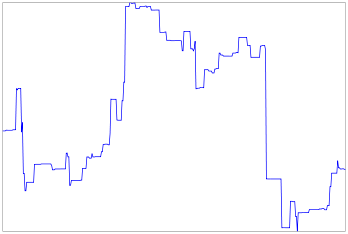
\includegraphics[width=\textwidth]{levy-sample-path}
      \caption{Типичная траектория процесса Леви}
      \label{fig:levy-sample-path}
    \end{figure}
  \end{columns}
\end{frame}

\begin{frame}{Генератор процесса Леви}
  Нетрудно убедиться, что переходные функции \( P_t (x, dy) \)
  процессов Леви порождают феллеровскую полугруппу в \( C_0
  \)
  \[
  ( T_t f ) ( x )
  = \int P_t ( x, \mathop{d y} ) f ( y ).
  \]

  Генератор этой полугруппы в общем случае задан может быть
  задан квадратичной формой
  \[
    \mathcal{E} ( u, v )
    = \int \frac{\partial u}{\partial x_i}
    \overline{\frac{\partial v}{\partial x_j}}
    \mathop{\mu_{i j} ( dx )}
    + \int \Big( u(x) - u(y) \Big)
    \overline{\left( v(x) - v(y) \right)}
    \mathop{J(dx dy)}
    + \int u(x) \overline{v(x)}
    \mathop{k(dx)}
  \]
  на области определения \( \mathcal{D}[\mathcal{E}] =
  C_0^\infty(D) \).

  \uncover<2->{
    Первое слагаемое обычно интерпретируется как вклад
    диффузии, второе -- как вклад скачков, а третье -- как
    поглощение в среде.
  }
\end{frame}

\begin{frame}{Приложения процессов Леви}
  \begin{itemize}
    \item Процессы Леви используются в финансовой математике чтобы
    моделировать распределения с длинными хвостами, возникающие
    в ходе эмпирического анализа так называемых
    \textit{стохастических процентных ставок}
    \[
      h_n = \ln \frac{S_n}{S_{n - 1}},
    \]
    где \( S_n \) -- это цена акции в момент времени \( n
    \). Подробнее в \cite{schiryaev-finance1}.
    \item Кроме того, процессы Леви возникают как естественные
      кандидаты в связи с описанием статистических эффектов
      \textit{долгой памяти}.
    \item Наконец, процессы Леви возникают в задачах теории
      массового обслуживания и теории запасов.
  \end{itemize}
\end{frame}

\bibliographystyle{babplain}
\bibliography{$BIB}

\end{document}
